\subsection{Arc length}

Let $g(t)$ be a function that draws a curve.
The arc length from $g(a)$ to $g(b)$ is given by
$$\int_a^b|g'(t)|\,dt$$
where $|g'(t)|$ is the length of the tangent vector at $g(t)$.
The integral sums over all of the tangent lengths to arrive at the total length
from $a$ to $b$.
For example, let us measure the length of the following curve.

{\color{blue}
\begin{verbatim}
xrange = (0,1)
yrange = (0,1)
draw(x^2)
\end{verbatim}}

\begin{center}
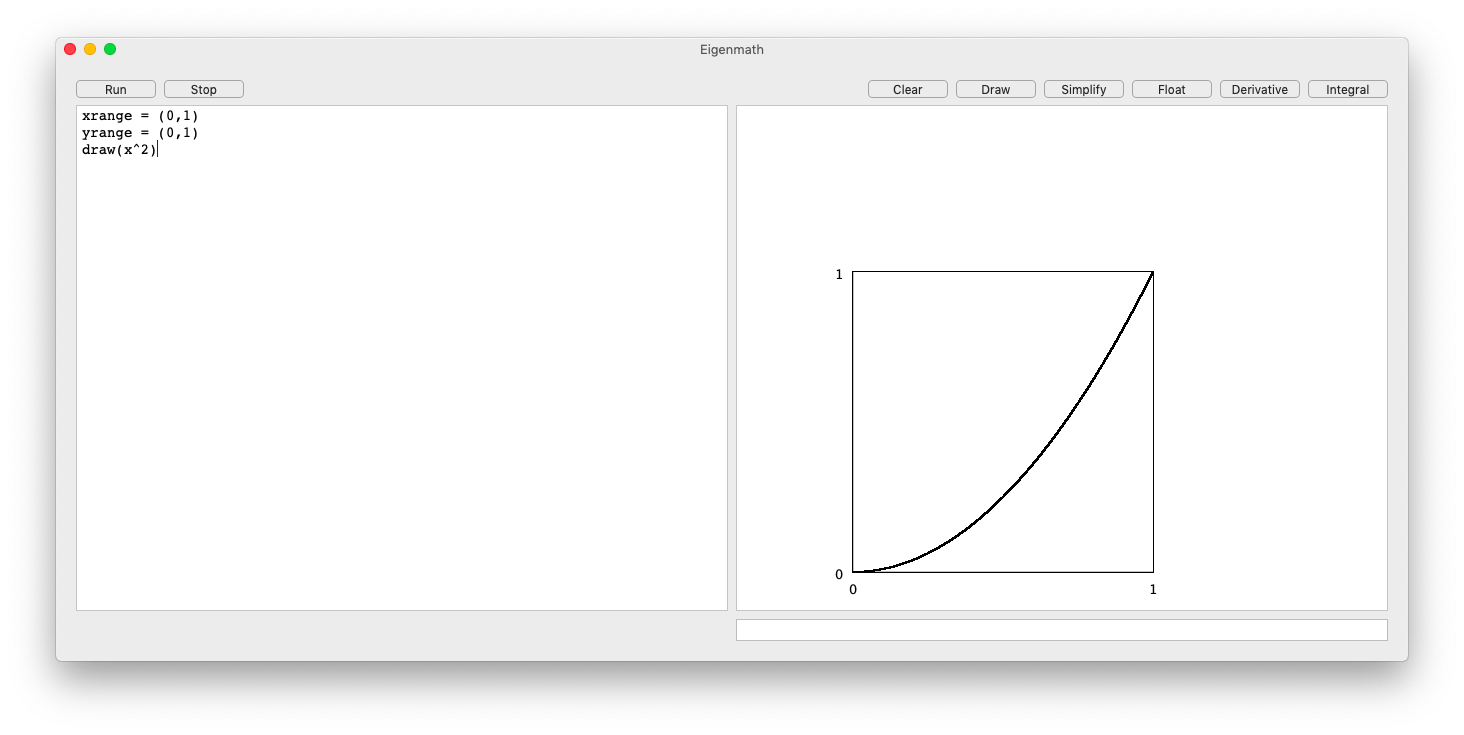
\includegraphics[scale=0.5]{arc.png}
\end{center}

\noindent
A suitable $g(t)$ for the arc is
$$g(t)=(t,t^2),\quad0\le t\le1$$
Hence one Eigenmath solution for computing the arc length is

\begin{Verbatim}[formatcom=\color{blue},samepage=true]
x = t
y = t^2
g = (x,y)
defint(abs(d(g,t)),t,0,1)
\end{Verbatim}

\noindent
$\displaystyle \tfrac{1}{2}\;5^{1/2}+\tfrac{1}{4}\log(5^{1/2}+2)$

\begin{Verbatim}[formatcom=\color{blue},samepage=true]
float
\end{Verbatim}

\noindent
$\displaystyle 1.47894$

\bigskip
\noindent
As expected, the result is greater than $\sqrt2\approx1.414$,
the length of the
diagonal from $(0,0)$ to $(1,1)$.

\bigskip
\noindent
The result seems rather complicated given that we
started with a simple parabola.
Let us inspect $|g'(t)|$ to see why.

\begin{Verbatim}[formatcom=\color{blue},samepage=true]
g
\end{Verbatim}

\noindent
$\displaystyle g=\begin{bmatrix}t\\ t^2\end{bmatrix}$

\begin{Verbatim}[formatcom=\color{blue},samepage=true]
d(g,t)
\end{Verbatim}

\noindent
$\displaystyle \begin{bmatrix}1\\ 2t\end{bmatrix}$

\begin{Verbatim}[formatcom=\color{blue},samepage=true]
abs(d(g,t))
\end{Verbatim}

\noindent
$\displaystyle (4t^2+1)^{1/2}$

\bigskip
\noindent
The following script does a discrete computation of the arc length
by dividing the curve into 100 pieces.

\begin{Verbatim}[formatcom=\color{blue},samepage=true]
g(t) = (t,t^2)
h(k) = abs(g(k/100.0) - g((k-1)/100.0))
sum(k,1,100,h(k))
\end{Verbatim}

\noindent
$\displaystyle 1.47894$

\bigskip
\noindent
As expected, the discrete result matches the analytic result.

\bigskip
\noindent
Find the length of the curve $y=x^{3/2}$ from the origin to
$x=\tfrac{4}{3}$.

\begin{Verbatim}[formatcom=\color{blue},samepage=true]
x = t
y = x^(3/2)
g = (x,y)
defint(abs(d(g,x)),x,0,4/3)
\end{Verbatim}

\noindent
$\displaystyle \tfrac{56}{27}$

\bigskip
\noindent
Because of the way $t$ is substituted for $x$,
the following code yields the same result.

\begin{Verbatim}[formatcom=\color{blue},samepage=true]
g = (t,t^(3/2))
defint(abs(d(g,t)),t,0,4/3)
\end{Verbatim}

\noindent
$\displaystyle \tfrac{56}{27}$

\subsection{Line integrals}
There are two different kinds of line integrals,
one for scalar fields and one
for vector fields.
The following table shows how both are based on the calculation of
arc length.

\begin{center}
\begin{tabular}{|l|l|l|}
\hline
& Abstract form
& Computable form
\\
\hline
 & &\\
Arc length
& $\displaystyle{\int_C ds}$
& $\displaystyle{\int_a^b |g'(t)|\,dt}$\\
 & &\\
\hline
 & & \\
Line integral, scalar field
& $\displaystyle{\int_C f\,ds}$
& $\displaystyle{\int_a^b f(g(t))\,|g'(t)|\,dt}$\\
& &\\
\hline
 & & \\
Line integral, vector field
& $\displaystyle{\int_C(F\cdot u)\,ds}$
& $\displaystyle{\int_a^b F(g(t))\cdot g'(t)\,dt}$\\
 & & \\
\hline
\end{tabular}
\end{center}

\noindent
For the vector field form, the symbol $u$ is the unit tangent vector
$$u=\frac{g'(t)}{|g'(t)|}$$
The length of the tangent vector cancels with $ds$
as follows.
$$\int_C(F\cdot u)\,ds
=\int_a^b\bigg(F(g(t))\cdot\frac{g'(t)}{|g'(t)|}\bigg)\,\bigg(|g'(t)|\,dt\bigg)
=\int_a^b F(g(t))\cdot g'(t)\,dt
$$

\noindent
Evaluate
$$\int_Cx\,ds\quad\hbox{and}\quad\int_Cx\,dx$$
where $C$ is a straight line from $(0,0)$ to $(1,1)$.

\bigskip
\noindent
What a difference the measure makes.
The first integral is over a scalar field and the second is over a vector field.
This can be understood when we recall that
$$ds=|g'(t)|\,dt
$$
Hence for $\int_Cx\,ds$ we have

\begin{Verbatim}[formatcom=\color{blue},samepage=true]
x = t
y = t
g = (x,y)
defint(x abs(d(g,t)),t,0,1)
\end{Verbatim}

\noindent
$\displaystyle \frac{1}{2^{1/2}}$

\bigskip
\noindent
For $\int_Cx\,dx$ we have

\begin{Verbatim}[formatcom=\color{blue},samepage=true]
x = t
y = t
g = (x,y)
F = (x,0)
defint(dot(F,d(g,t)),t,0,1)
\end{Verbatim}

\noindent
$\displaystyle \tfrac{1}{2}$

\bigskip
\noindent
The following line integral problems are from
{\it Advanced Calculus, Fifth Edition} by Wilfred Kaplan.

\bigskip
\noindent
Evaluate $\int y^2\,dx$ along the straight
line from $(0,0)$ to $(2,2)$.

\begin{Verbatim}[formatcom=\color{blue},samepage=true]
x = 2t
y = 2t
g = (x,y)
F = (y^2,0)
defint(dot(F,d(g,t)),t,0,1)
\end{Verbatim}

\noindent
$\displaystyle \tfrac{8}{3}$

\bigskip
\noindent
Evaluate $\int z\,dx+x\,dy+y\,dz$
along the path
$x=2t+1$, $y=t^2$, $z=1+t^3$, $0\le t\le 1$.

\begin{Verbatim}[formatcom=\color{blue},samepage=true]
x = 2t+1
y = t^2
z = 1+t^3
g = (x,y,z)
F = (z,x,y)
defint(dot(F,d(g,t)),t,0,1)
\end{Verbatim}

\noindent
$\displaystyle \tfrac{163}{30}$
